%!TEX root = ../main.tex

\section{Обобщение модели}

\subsection{Предложенное обобщение}

В ответ на описанную в предыдущем подразделе проблему в работе \cite{zipunova_higher_codimension}, на основании теоретических результатов работ \cite{sobolev_functional_analysis}, \cite{oleynik_biharmonic_equations}, \cite{sternin_elliptic_equations}, \cite{lewis_quasi_linear}, предлагается следующая обобщенная модель, для которой постановка условий на границах размерности 1 (соответственно, коразмерности 2) является математически корректной:
\begin{gather}
    \Pi = \int \limits_\Omega \pi d \vx \tcomma
    \label{eq:free_energy_corrected} \\
    \begin{aligned}
        \pi = -\half \epsilon[\phi] (\nabla \Phi, \nabla \Phi) + \Gamma \cfrac{1 - f(\phi)}{l^2} & + \cfrac{\Gamma}{4} (\nabla \phi, \nabla \phi) + \\ & + \alpha \cfrac{\Gamma l^2}{8} (\triangle \phi)^2 + \beta \cfrac{1}{p} \Gamma l^{p - 2} \| \, \nabla \phi \, \|_2^p \tsemicolon
    \end{aligned}
    \label{eq:free_energy_density_corrected}
\end{gather}
\begin{numcases}{}
    \Div(\epsilon[\phi] \nabla \Phi) = 0 \tsemicolon \label{equation_Phi_corrected} \\
    \begin{aligned}
        \cfrac{1}{m} \cfrac{\partial \phi}{\partial t} = \half \epsilon'(\phi) (\nabla \Phi, \nabla \Phi) & + \cfrac{\Gamma}{l^2} f'(\phi) + \half \Gamma \triangle \phi - \\ & - \alpha \cfrac{\Gamma l^2}{4} \triangle^2 \phi + \beta \Gamma l^{p - 2} \Div (\| \, \nabla \phi \, \|_2^{p - 2} \nabla \phi) \tpoint
    \end{aligned}
    \label{eq:phi_corrected}
\end{numcases}
Здесь $\alpha, \beta \geqslant 0$ -- некоторые константы, $p$ -- четное натуральное число, не меньшее~4. Дифференциальный оператор $\Div (\| \, \nabla \phi \, \|_2^{p - 2} \nabla \phi)$ принято называть \emph{$p$-лапласианом}, $\triangle^2 \phi = \triangle(\triangle \phi)$ -- \emph{билапласианом}. В дальнейшем для простоты будем считать $p = 4$.


\subsection{О методе конечных объемов}

Нашей целью будет численно исследовать систему уравнений \eqref{eq:Phi_corrected}, \eqref{eq:phi_corrected} в трех характеристических случаях, подобных описанному в подразделе \ref{subsection_matter_of_problem}.

Итак, мы ищем стационарное решение задачи \eqref{eq:Phi_corrected}, \eqref{eq:phi_corrected} с $\Phi \equiv 0$ для трех различных граничных условий:
\begin{enumerate}
    \item $\Omega = [0, +\infty)_x \times I_y \times I_z, \; \phi|_{x = 0} = 0, \; \phi \to 1$ при $x \to +\infty$ -- плоский случай;
    \item $\Omega = \Real_x \times \Real_y \times I_z, \; \phi|_{x, y = 0} = 0, \; \phi \to 1$ при $r = \sqrt{x^2 + y^2} \to +\infty$ -- цилиндрический случай;
    \item $\Omega = \Real_x \times \Real_y \times \Real_z, \; \phi|_{x, y, z = 0} = 0, \; \phi \to 1$ при $r = \sqrt{x^2 + y^2 + z^2} \to +\infty$ -- сферический случай.
\end{enumerate}
Подробно случаи 1 и 2 были описаны в подразделе \ref{subsection_matter_of_problem}. Случай 3 закономерно продолжает ряд: в нем граничное условие задано в точке -- объекте коразмерности 3.

Стационарное решение соответствует минимуму свободной энергии $\Pi$. Уравнения динамики системы выведены таковыми, что система стремится к минимуму энергии $\Pi$ в ходе эволюции. Поэтому будем проводить расчет на достаточно долгое время, тогда установившееся положение равновесия и будет искомым стационарным решением $\phi$.

В случаях 2 и 3 естественно перейти в цилиндрические и сферические координаты соответственно и считать решение $\phi$ зависящим только от радиуса $r$. В случае 1 для единообразия пространственную переменную также назовем $r$. Итак, $\phi(\vx) = \phi(r)$.

Для численного решения задачи воспользуемся методом конечных объемов. Классический метод конечных разностей, встречая ряд проблем, подходит плохо. К примеру, в уравнениях разностной схемы могут возникать ситуации деления на 0 в узле $r = 0$ в цилиндрическом и сферическом случае (см. формулу \eqref{eq:stationary_cylindrical}).

При моделировании мы ограничим область $\Omega$ некоторым конечным размером -- граничные условия превращаются в $\phi(0) = 0, \; \phi(R) = 1, \; R > 0$ -- внешний радиус $\Omega$, такой что $R / l \gg 1$.

Разобьем область $\Omega$ на $n + 1$ ячейку (прямоугольную либо в форме цилиндрического или сферического слоя), обозначим их $\Omega_0, ..., \Omega_n$. Пусть границы ячеек имеют радиусы $0 = r_{-1/2}, r_{1/2}, ..., r_{n + 1/2} = R$.

Обозначим $V(r)$ объем прямоугольника, цилиндра или сферы (в зависимости от случая), который заполняет область $\Omega$ от радиуса $0$ до $r$. Пусть $S(r)$ -- площадь внешней (разделяющей область $\Omega$) поверхности подобного прямоугольника, цилиндра или сферы. Тогда объем ячейки $\Omega_i$ равен $dV_i = V(r_{i + 1/2}) - V(r_{i - 1/2})$, площадь внутренней и внешней границ -- $S(r_{i - 1/2})$ и $S(r_{i + 1/2})$ соответственно.

\begin{enumerate}[label=\arabic*.]
    \item Плоский случай. $V(r) = r \cdot |I_y| \cdot |I_z|, \; S(r) = |I_y| \cdot |I_z|$. Сократив, можно считать $V(r) = r, \; S(r) = 1$.
    \item Цилиндрический случай. $V(r) = \pi r^2 \cdot |I_z|, \; S(r) = 2 \pi r \cdot |I_z|$. Сократив, можно считать $V(r) = r^2, \; S(r) = 2r$.
    \item Сферический случай. $V(r) = (4/3) \pi r^3, \; S(r) = 4 \pi r^2$. Домножив оба выражения на $3/(4\pi)$, можно считать $V(r) = r^3, \; S(r) = 3 r^2$.
\end{enumerate}

Итак, было показано, что можно считать $V(r) = r^{k + 1}, \; S(r) = (k + 1)r^k$, где $k = 0$ для плоского случая, $k = 1$ для цилиндрического, $k = 2$ для сферического.

Проведем преобразование решаемого уравнения \eqref{eq:phi_corrected}, обычное для метода конечных объемов. Учтем, что $\Phi \equiv 0$. Уравнение представляется в следующей форме:
\begin{equation}
    \cfrac{1}{m} \cfrac{\partial \phi}{\partial t} = \cfrac{\Gamma}{l^2} f'(\phi) + \Gamma \Div \overline{\rho} \tcomma
    \label{eq:phi_for_integration}
\end{equation}
где
$$\overline{\rho} = \half \nabla \phi - \alpha \cfrac{l^2}{4} \nabla (\triangle \phi) + \beta l^2 \| \, \nabla \phi \, \|_2^2 \nabla \phi \tpoint$$
Проинтегрируем уравнение \eqref{eq:phi_for_integration} вначале по некоторому промежутку времени [$t_j, t_{j + 1}]$, затем по ячейке $\Omega_i$. Преобразуем левую часть:
$$\int\limits_{\Omega_i} \int\limits_{t_j}^{t_{j + 1}} \cfrac{1}{m} \cfrac{\partial \phi}{\partial t} dt d \vx = \cfrac{1}{m} \int\limits_{\Omega_i} [\phi(\vx, t_{j + 1}) - \phi(\vx, t_j)] d \vx = \cfrac{dV_i}{m} [\widetilde{\phi}_i(t_{j + 1}) - \widetilde{\phi}_i(t_j)] \tcomma$$
где $\widetilde{\phi}_i$ -- это интегральное среднее функции $\phi$ по ячейке $\Omega_i$. Преобразуем правую часть, предварительно поменяв порядок интегрирования:
$$\int\limits_{t_j}^{t_{j + 1}} \int\limits_{\Omega_i} \left( \cfrac{\Gamma}{l^2} f'(\phi) + \Gamma \Div \overline{\rho} \right) d \vx dt = \int\limits_{t_j}^{t_{j + 1}} \left( \cfrac{\Gamma}{l^2} \int\limits_{\Omega_i} f'(\phi) d \vx + \Gamma \int\limits_{\partial \Omega_i} (\overline{\rho}, \overline{n}) dS \right) dt \tpoint$$
К интегралу слагаемого $\Gamma \Div \overline{\rho}$ была применена формула Гаусса--Остроградского. Функция $\phi$ зависит только от $r$, следовательно, вектор $\overline{\rho}$ всегда параллелен оси $r$. Граница ячейки $\partial \Omega_i$ складывается из внешней (где вектор нормали $\overline{n}$ и ось $r$ сонаправлены) и внутренней (где $\overline{n}$ и ось $r$ противоположно направлены). Обозначим $F_{i \pm 1/2}(t)$ поток в положительном направлении оси $r$ через соответствующую границу с радиусом $r_{i \pm 1/2}$:
$$F_{i \pm 1/2}(t) = \int\limits_{r = r_{i \pm 1/2}} (\overline{\rho}, \overline{n}) dS = \int\limits_{r = r_{i \pm 1/2}} \overline{\rho}_r dS = \overline{\rho}_r S(r_{i \pm 1/2}) = \rho_{i \pm 1/2}(t) \cdot S(r_{i \pm 1/2}) \tcomma$$
$$\int\limits_{\partial \Omega_i} (\overline{\rho}, \overline{n}) dS = F_{i + 1/2} - F_{i - 1/2} = \rho_{i + 1/2} S(r_{i + 1/2}) - \rho_{i - 1/2} S(r_{i - 1/2}) \tpoint$$
Здесь $\overline{\rho}_r$ обозначена $r$-координата вектора $\overline{\rho}$ (она же единственная ненулевая). Величину $\rho_{i \pm 1/2}(t) = \overline{\rho}_r(r_{i \pm 1/2}, t)$ будем называть плотностью потока через соответствующую границу. Таким образом, выведено следующее интегральное соотношение:
\begin{equation}
    \cfrac{dV_i}{m} [\widetilde{\phi}_i(t_{j + 1}) - \widetilde{\phi}_i(t_j)] = \int\limits_{t_j}^{t_{j + 1}} \left( \cfrac{\Gamma}{l^2} \int\limits_{\Omega_i} f'(\phi) d \vx + \Gamma \left[ \rho_{i + 1/2} S(r_{i + 1/2}) - \rho_{i - 1/2} S(r_{i - 1/2}) \right] \right) dt \tpoint
    \label{eq:finite_volume_integral}
\end{equation}

Первое слагаемое в подынтегральном выражении в правой части равенства \eqref{eq:finite_volume_integral} приблизим выражением $(\Gamma/l^2) \cdot dV_i \cdot f'[\widetilde{\phi}_i(t_j)]$. При построении разностной схемы от интеграла по $[t_j, t_{j + 1}]$ перейдем к умножению на $(t_{j + 1} - t_j)$ значения подынтегрального выражения в точке $t_j$.

Выясним, как вычислить плотность потока $\rho_{i \pm 1/2}$ во втором слагаемом. Если некоторая функция $\psi(\vx) = \psi(r)$, то
$$(\nabla \psi)_r = \cfrac{\partial \psi}{\partial r} \tcomma$$
где $\nabla \psi$ также зависит только от $r$. Таким образом:
\begin{equation}
    \rho = \half \cfrac{\partial \phi}{\partial r} - \alpha \cfrac{l^2}{4} \cfrac{\partial}{\partial r} (\triangle \phi) + \beta l^2 \left( \cfrac{\partial \phi}{\partial r} \right)^3 \tpoint
    \label{eq:finite_volumes_density}
\end{equation}

Традиционно в методе конечных объемов принимается, что локальное восполнение решения в ячейке -- постоянная функция. В силу того, что рассматриваемая задача требует постановки граничных условий при $r = 0$, а решение задачи вблизи этой точки может иметь большие производные, обобщим традиционный подход. А именно, будем считать, что в окрестности нуля решение представляется в виде линейной комбинации двух специально выбранных базисных функций, а его производные, соответственно, приближаются линейной комбинацией производных базисных функций с теми же коэффициентами. Опишем в общем виде поиск коэффициентов разложения.

Построим приближение для некоторой функции $\psi(r)$ в соседних ячейках $\Omega_i$ и $\Omega_{i + 1}$ по известным интегральным средним $\widetilde{\psi}_i$ и $\widetilde{\psi}_{i + 1}$ в этих ячейках. Пусть
$$g(r) = a \cdot g^{(a)}(r) + b \cdot g^{(b)} (r)$$
есть функция с двумя числовыми параметрами $a$ и $b$, $g^{(a)}$ и $g^{(b)}$ -- базисные функции, используемые для локального представления $\psi$. Найдем такие $a$ и $b$, что интегральные средние $g(r)$ по ячейкам $\Omega_i$ и $\Omega_{i + 1}$ были бы равны $\widetilde{\psi}_i$ и $\widetilde{\psi}_{i + 1}$ соответственно. Это эквивалентно системе уравнений
\begin{numcases}{}
    \int\limits_{r_{i - 1/2}}^{r_{i + 1/2}} [\widetilde{\psi}_i - g(r)] S(r) dr = 0 \tsemicolon
    \label{eq:interpolation_first} \\
    \int\limits_{r_{i + 1/2}}^{r_{i + 3/2}} [\widetilde{\psi}_{i + 1} - g(r)] S(r) dr = 0 \tpoint
    \label{eq:interpolation_second}
\end{numcases}
Пусть
$$\int\limits_{r_{i - 1/2}}^{r_{i + 1/2}} g^{(a)}(r) S(r) dr = I_i^{(a)}; \qquad \int\limits_{r_{i - 1/2}}^{r_{i + 1/2}} g^{(b)}(r) S(r) dr = I_i^{(b)} \tpoint$$
Считаем, что интегралы $I_i^{(a)}$ и $I_i^{(b)}$ найдены аналитически. Тогда система \eqref{eq:interpolation_first}, \eqref{eq:interpolation_second} эквивалентна системе
$$\begin{cases}
    a I_i^{(a)} + b I_i^{(b)} = (r_{i + 1/2}^{k + 1} - r_{i - 1/2}^{k + 1}) \widetilde{\psi}_i \tsemicolon \\
    a I_{i + 1}^{(a)} + b I_{i + 1}^{(b)} = (r_{i + 3/2}^{k + 1} - r_{i + 1/2}^{k + 1}) \widetilde{\psi}_{i + 1} \tpoint
\end{cases}$$
Это система двух линейных уравнений с двумя неизвестными -- решим методом Крамера. Получим:
$$\varDelta = I_i^{(a)} I_{i + 1}^{(b)} - I_i^{(b)} I_{i + 1}^{(a)} \tsemicolon$$
\begin{equation}
    a = \cfrac{(r_{i + 1/2}^{k + 1} - r_{i - 1/2}^{k + 1}) I_{i + 1}^{(b)}}{\varDelta} \cdot \widetilde{\psi}_i + \cfrac{-(r_{i + 3/2}^{k + 1} - r_{i + 1/2}^{k + 1}) I_i^{(b)}}{\varDelta} \cdot \widetilde{\psi}_{i + 1} \tsemicolon
    \label{eq:interpolation_a}
\end{equation}
\begin{equation}
    b = \cfrac{-(r_{i + 1/2}^{k + 1} - r_{i - 1/2}^{k + 1}) I_{i + 1}^{(a)}}{\varDelta} \cdot \widetilde{\psi}_i + \cfrac{(r_{i + 3/2}^{k + 1} - r_{i + 1/2}^{k + 1}) I_i^{(a)}}{\varDelta} \cdot \widetilde{\psi}_{i + 1} \tpoint
    \label{eq:interpolation_b}
\end{equation}
Теперь можно легко находить $a$ и $b$ при различных значениях $\widetilde{\psi}_i, \; \widetilde{\psi}_{i + 1}$, если вычислить заранее и сохранить четыре коэффициента, стоящие в формулах \eqref{eq:interpolation_a}, \eqref{eq:interpolation_b}. 

Приблизим $\partial \psi / \partial r$ на границе с радиусом $r_{i + 1/2}$ (между ячейками $\Omega_i$ и $\Omega_{i + 1}$) с помощью функции $g(r)$ с известными числовыми параметрами:
$$\left[ \cfrac{\partial \psi}{\partial r} \right]_{i + 1/2} = g'(r_{i + 1/2}) = a \cdot (g^{(a)})'(r_{i + 1/2}) + b \cdot (g^{(b)})'(r_{i + 1/2}) \tpoint$$
Производные $(g^{(a)})'$ и $(g^{(b)})'$ считаем найденными аналитически.

Отыщем приближение производной $\partial \phi / \partial r$ на границах с радиусами $r_{3/2}, ...$, $r_{n - 1/2}$ (то есть на всех, кроме первых двух внутренних и крайней внешней). Используем описанный выше метод с $\widetilde{\psi} = \widetilde{\phi}$ и базисными функциями $g^{(a)}(r) = r, \; g^{(b)}(r) = 1$. $g' \equiv a$, вывести формулы для $I^{(a)}$, $I^{(b)}$ также не составляет труда. Таким образом, происходит приближение функции $\phi$ на парах соседних ячеек линейной функцией.

Задание граничных условий, в том числе приближение $\partial \phi / \partial r$ на крайних границах $\Omega$, будет подробно описано в следующем разделе.

Без ответа остался только вопрос вычисления $\triangle \phi$ и его производной по $r$. Оно требуется лишь в случае ненулевой константы $\alpha$ (см. уравнение \eqref{eq:phi_corrected}). Проведя рассуждение, аналогичное проделанному для вывода соотношения \eqref{eq:finite_volume_integral}, но без интегрирования по времени, получим следующее выражение для интегрального среднего лапласиана $\phi$ по ячейке:
\begin{equation}
    dV_i \cdot \widetilde{\triangle \phi}_i = \cfrac{\partial \phi}{\partial r} \bigg|_{r = r_{i + 1/2}} S(r_{i + 1/2}) - \cfrac{\partial \phi}{\partial r} \bigg|_{r = r_{i - 1/2}} S(r_{i - 1/2}) \tpoint
    \label{eq:finite_volume_laplasian}
\end{equation}

По средним $\widetilde{\triangle \phi}$ вычислим приближение $\partial (\triangle \phi) / \partial r$ на границах ячеек с радиусами $r_{1/2}, ..., r_{n - 1/2}$ (то есть на всех, кроме крайних внутренней и внешней) тем же способом, который ранее использовался для $\partial \phi / \partial r$, с $\widetilde{\psi} = \widetilde{\triangle \phi}, \; g^{(a)}(r) = r, \; g^{(b)}(r) = 1$.


\subsection{Задание граничных условий}

Граничные условия, подробно описанные в предыдущем разделе, имеют следующий вид: $\phi(0) = 0, \; \phi(R) = 1, \; R > 0$, где $R$ такое, что $R / l \gg 1$. Если коэффициент $\alpha$ в уравнении \eqref{eq:phi_corrected} при слагаемом с билапласианом ненулевой, то этих граничных условий недостаточно в силу повышения порядка уравнения -- необходимо добавить условия на производные. По логике задачи их следует сделать таковыми:
$$\cfrac{\partial \phi}{\partial r} \bigg|_{r = 0} = 0, \qquad \cfrac{\partial \phi}{\partial r} \bigg|_{r = 1} = 0 \tpoint$$

Граничные условия в точке $r = R$ в разностной схеме задаются легко: $\widetilde{\phi}_n \equiv 1, \; \widetilde{\triangle \phi}_n \equiv 0$. Этого оказывается достаточно ввиду того, что функция $\phi$ вблизи точки $R$ меняется очень слабо.

С граничными условиями в точке $r = 0$ дела обстоят намного сложнее. Для начала, функции перехода в цилиндрическую и сферическую систему координат имеют в этой точке особенность. К тому же ожидается, что $\phi$ в окрестности точки $r = 0$ довольно быстро растет. Более того, как выяснится позже, в цилиндрическом и сферическом случае в точке $0$ имеют особенность производные функций $\phi$ и $\triangle \phi$.

Зададим граничные условия в точке $0$ следующим образом. Выберем для приближения $\phi$ в ячейках $\Omega_0$ и $\Omega_1$ такие базисные функции $g^{(a)}$ и $g^{(b)}$, что каждая из них удовлетворяет граничным условиям при $r = 0$ и, при необходимости, одна из них имеет в точке $0$ предположительно тот же вид особенности, что решение $\phi$. С помощью функции $g(r)$ с известными параметрами получим искомые приближения:
$$\left[ \cfrac{\partial \phi}{\partial r} \right]_{-1/2} = g'(0); \qquad \left[ \cfrac{\partial \phi}{\partial r} \right]_{1/2} = g'(r_{1/2}) \tsemicolon$$
$$\left[ \cfrac{\partial (\triangle \phi)}{\partial r} \right]_{-1/2} = \cfrac{\partial}{\partial r} \left[ r^k \cfrac{\partial}{\partial r} \left(\cfrac{1}{r^k} \cfrac{\partial g}{\partial r} \right) \right] \Bigg|_{r = 0} \tpoint$$
В последнем выражении используется общий вид формулы для лапласиана функции, зависящей только от $r$, в прямоугольных, цилиндрических и сферических координатах:
\begin{equation}
    \triangle g = \cfrac{1}{r^k} \cfrac{\partial}{\partial r} \left( r^k \cfrac{\partial g}{\partial r} \right) \tpoint
    \label{eq:laplasian_common}
\end{equation}

Определимся с выбором базисных функций для приближения $\phi$ в первых двух ячейках в зависимости от случая задачи и значений параметров $\alpha$ и $\beta$.

Рассмотрим плоский случай. Здесь у производной $\phi$ (и $\triangle \phi$, входящей в формулы, только если $\alpha \neq 0$) в точке $0$ не ожидается особенностей. Обоснуем это так: $S(0) = 1 \neq 0$, поэтому для ненулевого потока $F_{-1/2}$ через крайнюю внутреннюю границу нужна ненулевая конечная плотность потока $\rho_{-1/2}$. При $\alpha = 0$ граничное условие $\phi(0) = 0$ -- возьмем $g^{(a)} = r^2, \; g^{(b)} = r$. При $\alpha \neq 0$ добавляется граничное условие $\partial \phi / \partial r |_{r = 0} = 0$ -- используем $g^{(a)} = r^3, \; g^{(b)} = r^2$.

Теперь рассмотрим цилиндрический случай. Имеем $S(0) = 0$, поэтому, казалось бы, поток $F_{-1/2}$ всегда нулевой. Однако если допустить у $\rho$ особенность вида $1/r$, то получается $\rho(r) S(r) \to 2$ при $r \to +0$ -- конечный ненулевой поток! Если $\rho$ по модулю растет асимптотически медленнее, то поток будет нулевым, если быстрее, то бесконечным (что не имеет смысла).

Пусть $\alpha = \beta = 0$. Тогда в выражении \eqref{eq:finite_volumes_density} для плотности потока встречается лишь $\partial \phi / \partial r$ в первой степени. Значит, мы ищем $g^{(a)}$, такую что $(g^{(a)})' = C_0/r$. Проинтегрировав, получим $g^{(a)} = C_0 \ln r + C_1$. $g^{(a)} \to \infty$ при $r \to +0$, то есть граничное условие $g^{(a)}(0) = 0$ выполнить невозможно. Это косвенно подтверждает вывод из работы \cite{zipunova_higher_codimension}, что в этом случае решения дифференциальной задачи не существует.

Пусть $\alpha = 0, \; \beta \neq 0$. В выражение \eqref{eq:finite_volumes_density} для плотности потока входит $\partial \phi / \partial r$ в первой и третьей степени. Следовательно, мы ищем $g^{(a)}$, такую что $(g^{(a)})' = C_0 r^{-1/3}$. Ее первая степень даст нулевой вклад в поток, а третья -- конечный ненулевой. Проинтегрировав, получим $g^{(a)} = C_0 \cdot (3/2) \cdot r^{2/3} + C_1$. С учетом граничного условия выберем $g^{(a)} = r^{2/3}$. Вторую базисную функцию возьмем без особенности в точке $0$, например, $g^{(b)} = r$.

Пусть $\alpha \neq 0, \; \beta$ произвольное. Тогда в выражение \eqref{eq:finite_volumes_density} для плотности потока входит $\partial (\triangle \phi) / \partial r$. Встречается там и $\partial \phi / \partial r$, но она, согласно граничному условию, равна~$0$ при $r = 0$. Отыщем такую базисную функцию $g^{(a)}$, что $\partial (\triangle g^{(a)}) / \partial r = C_0 / r$. Учтем, что лапласиан функции $g^{(a)}$, зависящей только от $r$, в цилиндрических координатах вычисляется по формуле \eqref{eq:laplasian_common} с $k = 1$. Трижды проинтегрировав уравнение на производную лапласиана, получим $g^{(a)} = (C_0/4) r^2 (\ln r - 1) + C_1 r^2 / 4 + C_2 \ln r + C_3$. Требуется $g^{(a)}(0) = 0$, следовательно, $C_2 = C_3 = 0$. Особенность содержит первое слагаемое, поэтому выберем $g^{(a)} = r^2 (\ln r - 1)$. $g^{(a)}$ удовлетворяет граничному условию на производную $\partial g^{(a)} / \partial r|_{r = 0} = 0$. Второй базисной функцией сделаем $g^{(b)} = r^2$.

Наконец, рассмотрим сферический случай. Аналогично цилиндрическому случаю будем подбирать базисную функцию так, чтобы поток $F_{-1/2}$ был конечным. Для этого $\rho$ должна иметь особенность вида $1/r^2$, так как тогда $\rho(r) S(r) \to 3$ при $r \to 0$.

Пусть $\alpha = \beta = 0$. Аналогично рассмотренному ранее случаю ищем $g^{(a)}$, такую что $(g^{(a)})' = C_0 / r^2$. Проинтегрировав, получим $g^{(a)} = -C_0 / r + C_1$. $g^{(a)} \to \infty$ при $r \to +0$, то есть граничное условие $g^{(a)}(0) = 0$ выполнить невозможно.

Пусть $\alpha = 0, \; \beta \neq 0$. Аналогично рассмотренному ранее случаю ищем $g^{(a)}$, такую что $(g^{(a)})' = C_0 / r^{-2/3}$. Проинтегрировав, получим $g^{(a)} = C_0 \cdot 3 \cdot r^{1/3} + C_1$. С учетом граничного условия выберем $g^{(a)} = r^{1/3}, \; g^{(b)} = r$.

Пусть $\alpha \neq 0, \; \beta$ произвольное. Аналогично рассмотренному ранее случаю ищем $g^{(a)}$, такую что $\partial (\triangle g^{(a)}) / \partial r = C_0 / r^2$. Лапласиан функции $g^{(a)}$, зависящей только от $r$, в сферических координатах вычисляется по формуле \eqref{eq:laplasian_common} с $k = 2$. Дважды проинтегрировав уравнение на производную лапласиана, получим $(g^{(a)})' = -C_0 / 2 + C_1 r / 3 + C_2 / r^2$. $C_0 \neq 0$, так как иначе у функции пропадет особенность. Получается, что $(g^{(a)})'(0) \neq 0$ -- невозможно удовлетворить граничному условию на производную!

Примечательно, что выбранный подход не удалось применить в сферическом случае не только при $\alpha = \beta = 0$, но и при $\alpha \neq 0$. Выдвинем гипотезу, что в обеих этих конфигурациях исследуемая дифференциальная задача поставлена некорректно и не имеет решения.


\subsection{Разностная схема}

Везде в двух предыдущих подразделах допускалось, что радиусы границ ячеек $0 = r_{-1/2}, r_{1/2}, ..., r_{n - 1/2}, r_{n + 1/2} = R$ могут быть произвольной возрастающей последовательностью чисел. В дальнейшем, на практике, мы сделаем их структуру регулярной с шагом $h$: $r_{i - 1/2} = ih$.

При моделировании система будет проходить моменты времени $t_j = j \tau$, где $\tau$ -- фиксированный шаг по времени. Функцию времени с аргументом $t_j$ будем обозначать верхним индексом $j$.

В качестве начального условия задаются $\{ \widetilde{\phi}_i^0 \}_{i = 0}^n$.

Как было принято ранее, $k = 0$ в плоском случае, $k = 1$ в цилиндрическом, $k = 2$ в сферическом.

Подводя итог рассуждениям, проделанным в двух предыдущих подразделах, выпишем построенную методом конечных объемов разностную схему.

\begin{equation}
    \begin{gathered}
        \cfrac{1}{m} (\widetilde{\phi}_i^{j + 1} - \widetilde{\phi}_i^j) = \tau \cfrac{\Gamma}{l^2} f'(\widetilde{\phi}_i^j) + \cfrac{\tau}{dV_i} \Gamma (\rho_{i + 1/2}^j S_{i + 1/2} - \rho_{i - 1/2}^j S_{i - 1/2}) \; \text{при} \; i = \overline{0, n - 1} \tsemicolon \\
        \widetilde{\phi}_n^j = 1 \tsemicolon
    \end{gathered}
    \label{sch:volime_phi}
\end{equation}
$$dV_i = r_{i + 1/2}^{k + 1} - r_{i - 1/2}^{k + 1}; \qquad S_{i \pm 1/2} = (k + 1) r_{i \pm 1/2}^k \tsemicolon$$
\begin{equation}
    \rho_{i \pm 1/2}^j = \half \left[ \cfrac{\partial \phi}{\partial r} \right]_{i \pm 1/2}^j - \alpha \cfrac{l^2}{4} \left[ \cfrac{\partial (\triangle \phi)}{\partial r} \right]_{i \pm 1/2}^j + \beta l^2 \left( \left[ \cfrac{\partial \phi}{\partial r} \right]_{i \pm 1/2}^j \right)^3 \tsemicolon
    \label{sch:volume_density}
\end{equation}
\begin{equation}
    \left[ \cfrac{\partial \phi}{\partial r} \right]_{i + 1/2}^j = a_{i + 1/2}^j \; \text{при} \; i = \overline{1, n - 1} \tsemicolon
    \label{sch:volume_phi_derivative}
\end{equation}
$$\{\widetilde{\phi}_i^j\}_{i = 1}^n \leadsto \{a_{i + 1/2}^j\}_{i = 1}^{n - 1}, \; \text{где} \; g^{(a)} = r, \; g^{(b)} = 1 \tsemicolon$$
\begin{equation}
    \begin{gathered}
        \widetilde{\triangle \phi}_i^j = \cfrac{1}{dV_i} \left( \left[ \cfrac{\partial \phi}{\partial r} \right]_{i + 1/2}^j S_{i + 1/2} - \left[ \cfrac{\partial \phi}{\partial r} \right]_{i - 1/2}^j S_{i - 1/2} \right) \; \text{при} \; i = \overline{0, n - 1} \tsemicolon \\
        \widetilde{\triangle \phi}_n^j = 0 \tsemicolon
    \end{gathered}
    \label{sch:volume_laplasian}
\end{equation}
\begin{equation}
    \left[ \cfrac{\partial (\triangle \phi)}{\partial r} \right]_{i + 1/2}^j = c_{i + 1/2}^j \; \text{при} \; i = \overline{0, n - 1} \tsemicolon
    \label{sch:volume_laplasian_derivative}
\end{equation}
$$\{\widetilde{\triangle \phi}_i^j\}_{i = 0}^n \leadsto \{c_{i + 1/2}^j\}_{i = 0}^{n - 1}, \; \text{где} \; g^{(c)} = r, \; g^{(d)} = 1 \tsemicolon$$
\begin{equation}
    \left[ \cfrac{\partial \phi}{\partial r} \right]_{i - 1/2}^j = a_{1/2}^j (g_{1/2}^{(a)})'(r_{i - 1/2}) + b_{1/2}^j (g_{1/2}^{(b)})'(r_{i - 1/2}) \; \text{при} \; i = \overline{0, 1} \tsemicolon
    \label{sch:volume_phi_derivetive_border}
\end{equation}
\begin{equation}
    \left[ \cfrac{\partial (\triangle \phi)}{\partial r} \right]_{-1/2}^j = a_{1/2}^j \cfrac{\partial (\triangle g^{(a)})}{\partial r} \bigg|_{r = 0} + b_{1/2}^j \cfrac{\partial (\triangle g^{(b)})}{\partial r} \bigg|_{r = 0} \tsemicolon
    \label{sch:volume_laplasian_derivative_border}
\end{equation}
$$\{ \widetilde{\phi}_0^j, \widetilde{\phi}_1^j \} \leadsto \{ a_{1/2}^j, b_{1/2}^j \} \tpoint$$
1. Плоский случай при $\alpha = 0$:
\begingroup
\setlength{\abovedisplayskip}{5pt}
\setlength{\belowdisplayskip}{5pt}
\begin{align*}
    g_{1/2}^{(a)} &= r^2, & (g_{1/2}^{(a)})' &= 2r, & I^{(a)} &= \cfrac{1}{3} r^3 \bigg|_{...}^{...} \tsemicolon \\
    g_{1/2}^{(b)} &= r, & (g_{1/2}^{(b)})' &= 1, & I^{(b)} &= \half r^2 \bigg|_{...}^{...} \tpoint
\end{align*}
2. Плоский случай при $\alpha \neq 0$:
\begin{align*}
    g_{1/2}^{(a)} &= r^3, & (g_{1/2}^{(a)})' &= 3r^2, & \cfrac{\partial (\triangle g_{1/2}^{(a)})}{\partial r} &= 6, & I^{(a)} &= \cfrac{1}{4} r^4 \bigg|_{...}^{...} \tsemicolon \\
    g_{1/2}^{(b)} &= r^2, & (g_{1/2}^{(b)})' &= 2r, & \cfrac{\partial (\triangle g_{1/2}^{(b)})}{\partial r} &= 0, & I^{(b)} &= \cfrac{1}{3} r^3 \bigg|_{...}^{...} \tpoint
\end{align*}
3. Цилиндрический случай при $\alpha = 0, \; \beta \neq 0$:
\begin{align*}
g_{1/2}^{(a)} &= r^{2/3}, & (g_{1/2}^{(a)})' &= \cfrac{2}{3} r^{-1/3}, & I^{(a)} &= \cfrac{3}{4} r^{8/3} \bigg|_{...}^{...} \tsemicolon \\
g_{1/2}^{(b)} &= r, & (g_{1/2}^{(b)})' &= 1, & I^{(b)} &= \cfrac{2}{3} r^3 \bigg|_{...}^{...} \tsemicolon
\end{align*}
$$\rho_{-1/2}^j S_{-1/2} = \cfrac{16}{27} (a_{1/2}^j)^3 \tpoint$$
4. Цилиндрический случай при $\alpha \neq 0$:
\begin{align*}
    g_{1/2}^{(a)} &= r^2 (\ln r - 1), & (g_{1/2}^{(a)})' &= r (2 \ln r - 1), & \cfrac{\partial (\triangle g_{1/2}^{(a)})}{\partial r} &= \cfrac{4}{r}, & I^{(a)} &= \cfrac{1}{8} r^4 (4 \ln r - 5) \bigg|_{...}^{...} \tsemicolon \\
    g_{1/2}^{(b)} &= r^2, & (g_{1/2}^{(b)})' &= 2r, & \cfrac{\partial (\triangle g_{1/2}^{(a)})}{\partial r} &= 0, & I^{(b)} &= \half r^4 \bigg|_{...}^{...} \tsemicolon
\end{align*}
$$\left[ \cfrac{\partial (\triangle \phi)}{\partial r} \right]_{-1/2}^j S_{-1/2} = 8 a_{1/2}^j \tpoint$$
5. Сферический случай при $\alpha = 0, \; \beta \neq 0$:
\begin{align*}
    g_{1/2}^{(a)} &= r^{1/3}, & (g_{1/2}^{(a)})' &= \cfrac{1}{3} r^{-2/3}, & I^{(a)} &= \cfrac{9}{10} r^{10/3} \bigg|_{...}^{...}  \tsemicolon \\
    g_{1/2}^{(b)} &= r, & (g_{1/2}^{(b)})' &= 1, & I^{(b)} &= \cfrac{3}{4} r^4 \bigg|_{...}^{...} \tsemicolon
\end{align*}
$$\rho_{-1/2}^j S_{-1/2} = \cfrac{1}{9} (a_{1/2}^j)^3 \tpoint$$
\endgroup


\subsection{Вычислительный эксперимент}

Была написана программа, реализующая разностную схему \eqref{sch:volime_phi}, \eqref{sch:volume_density}, \eqref{sch:volume_phi_derivative}, \eqref{sch:volume_laplasian}, \eqref{sch:volume_laplasian_derivative}, \eqref{sch:volume_phi_derivetive_border}, \eqref{sch:volume_laplasian_derivative_border}.

Все предыдущие рассуждения были универсальны для плоского, цилиндрического и сферического случаев, насколько это возможно. Все три случая моделируются одной и той же программой, принимающей $k = \overline{0, 2}$ как параметр.

Зададим параметры модели:
$$\epsilon_0 = 0.2, \; \delta = 0.04, \; l = 1.0, \; \Gamma = 1.0, \; m = 0.5 \tpoint$$

Пусть $R = 5$. По виду графиков будет понятно, что для использованного набора параметров такое $R$ достаточно велико.

Выберем число ячеек $n = 300$ при $\alpha = 0$ и $n = 150$ иначе. Шаг по пространству~$h$, соответственно, равен $1/30 \approx 0.0333$ либо $1/60 \approx 0.0167$. При этом придется брать шаг по времени $\tau = 5 \cdot 10^{-7}$. Если шаг по времени кратно больше, то схема оказывается неустойчива и программа завершается с ошибкой переполнения (в данных возникает значение NaN). Как и ожидалось, $p$-лапласиан и билапласиан (особенно) требуют относительно малых шагов по времени.

Выбор начальных условий не имеет значения. Пусть, например, значения $0$ и $1$ гладко соединяются ветвью синусоиды: $\widetilde{\phi}_i^0 = \sin[(h/2 + ih) \pi / 2], \; h/2 + ih < 1$; далее все значения равны $1$.

Будем останавливать расчет, когда вектор <<воздействия>> на систему достаточно мал, а именно:
$$\max\limits_{i = 0}^n \cfrac{\widetilde{\phi}_i^{j + 1} - \widetilde{\phi}_i^j}{m} < 10^{-9} \tpoint$$
Все конфигурации модели достигли названного условия не более чем через $7.4$ единицы времени.

Результаты вычислений изображены на рис. \ref{fig:result_volumes} и \ref{fig:result_volumes_p} (случай 1 из описания разностной схемы), рис. \ref{fig:result_volumes_bi} (случай 2), рис. \ref{fig:result_volumes_cyl_p} (случай 3), рис. \ref{fig:result_volumes_cyl_bi} (случай 4), рис.~\ref{fig:result_volumes_sph_p} (случай~5). Графики функций показаны до зримого момента выхода на примерно постоянное значение $1$, после чего они в действительности продолжаются до $R = 5$. Графики состоят из соединенных значений средних $\widetilde{\phi}_i^j$, размещенных в серединах ячеек; вблизи~$0$ к ним добавлено несколько значений приближающей функции $g^{(a)}$, имеющей особенность в $0$, если того требует случай задачи.

\begin{figure}[!tp]
    \centering
    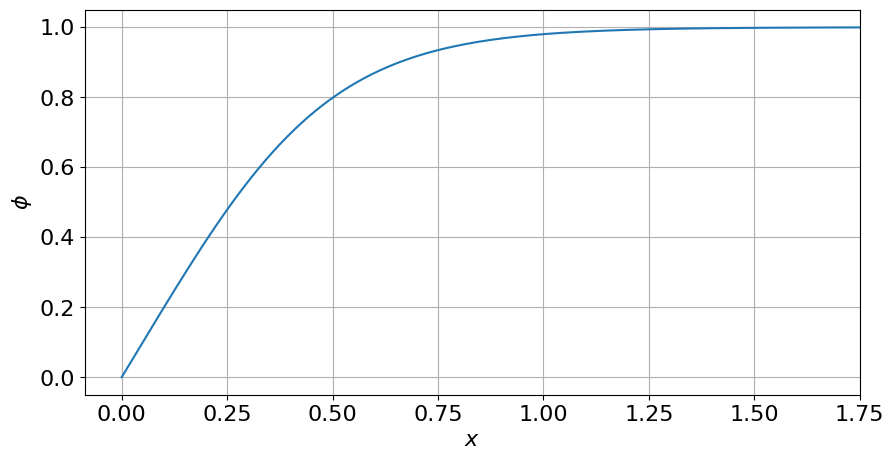
\includegraphics[width=0.89\textwidth]{figures/result_volumes.png}
    \vspace{-0.3cm}
    \caption{Решение $\phi$ в плоском случае при $\alpha = 0, \; \beta = 0$.}
    \label{fig:result_volumes}
    \vspace{0.5cm}

    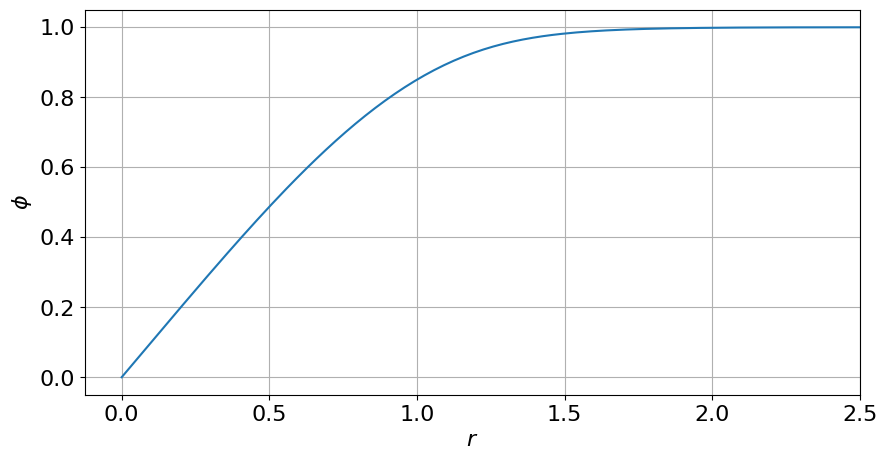
\includegraphics[width=0.89\textwidth]{figures/result_volumes_p.png}
    \vspace{-0.3cm}
    \caption{Решение $\phi$ в плоском случае при $\alpha = 0, \; \beta = 1$.}
    \label{fig:result_volumes_p}
    \vspace{0.5cm}
    
    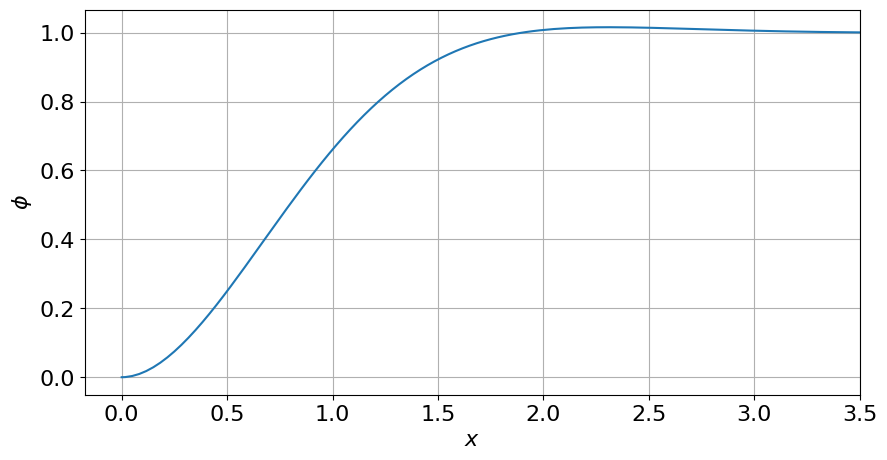
\includegraphics[width=0.89\textwidth]{figures/result_volumes_bi.png}
    \vspace{-0.3cm}
    \caption{Решение $\phi$ в плоском случае при $\alpha = 1, \; \beta = 0$.}
    \label{fig:result_volumes_bi}
\end{figure}

\begin{figure}[!tp]
    \centering
    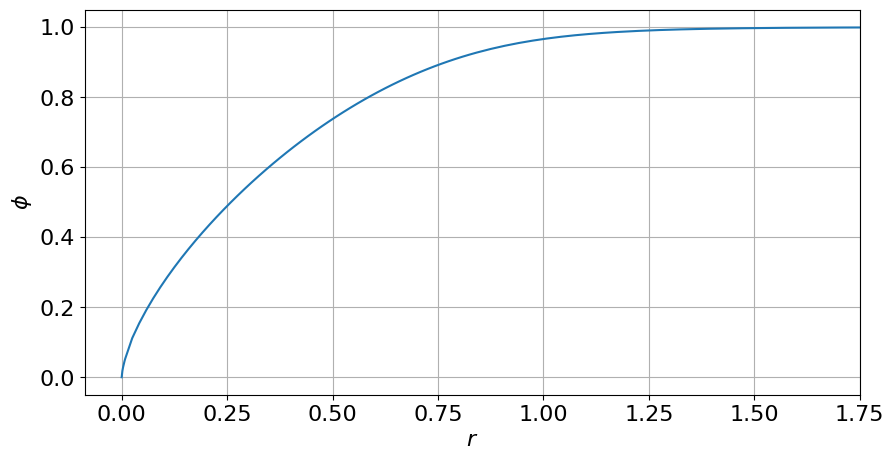
\includegraphics[width=0.89\textwidth]{figures/result_volumes_cyl_p.png}
    \vspace{-0.3cm}
    \caption{Решение $\phi$ в цилиндрическом случае при $\alpha = 0, \; \beta = 1$.}
    \label{fig:result_volumes_cyl_p}
    \vspace{0.5cm}

    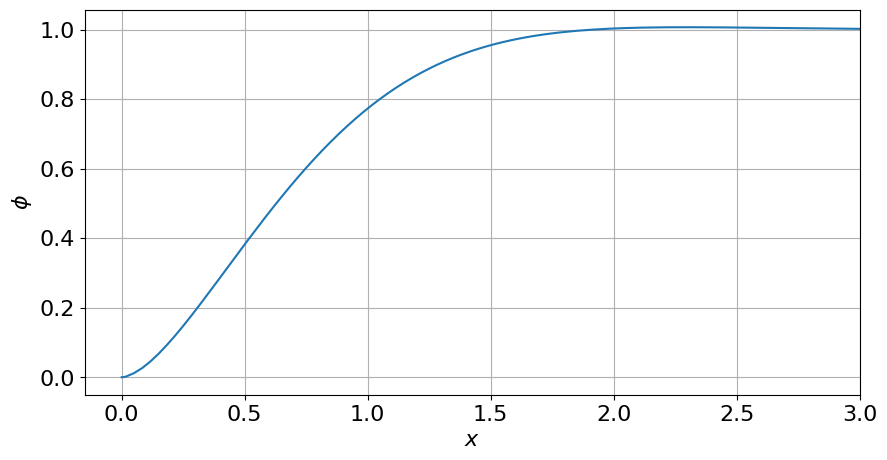
\includegraphics[width=0.89\textwidth]{figures/result_volumes_cyl_bi.png}
    \vspace{-0.3cm}
    \caption{Решение $\phi$ в цилиндрическом случае при $\alpha = 1, \; \beta = 0$.}
    \label{fig:result_volumes_cyl_bi}
    \vspace{0.5cm}
    
    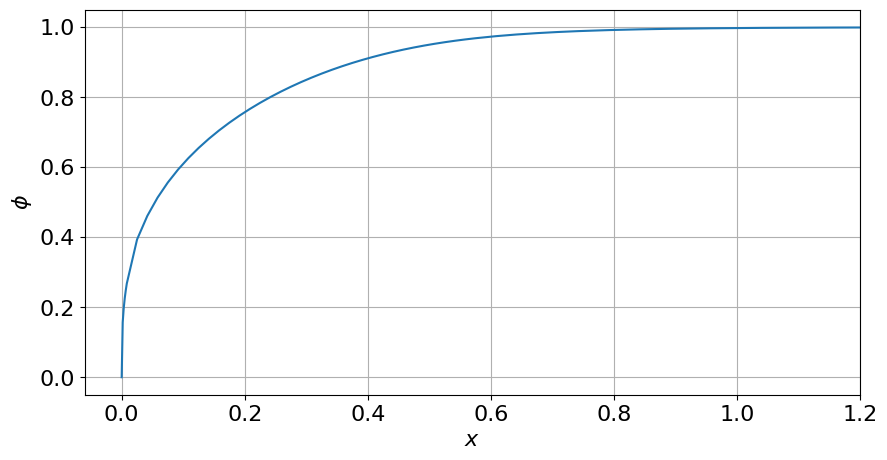
\includegraphics[width=0.89\textwidth]{figures/result_volumes_sph_p.png}
    \vspace{-0.3cm}
    \caption{Решение $\phi$ в сферическом случае при $\alpha = 0, \; \beta = 1$.}
    \label{fig:result_volumes_sph_p}
\end{figure}

Отметим, что если в уравнения входит билапласиан ($\alpha \neq 0$), то функция $\phi$ может быть не монотонной и в некоторых точках превышать значение $1$ (см. рис. \ref{fig:result_volumes_bi}, \ref{fig:result_volumes_cyl_bi}). В работе \cite{zipunova_higher_codimension} это было отмечено и указано, что монотонность $\phi$ следует ожидать при достаточно малых $\alpha$.

Итак, эксперимент подтверждает, что, несмотря на некоторую громоздкость формулировок, предложенная модификация метода конечных объемов позволяет эффективно моделировать решение $\phi$, даже если на границе области оно имеет особенность.